\documentclass[tikz,border=6pt]{standalone}
\usepackage[T1]{fontenc}
\usepackage{lmodern}
\usepackage{xcolor}
\usetikzlibrary{arrows.meta,positioning}

\definecolor{SlateText}{HTML}{23364D}
\definecolor{SlateLine}{HTML}{60758A}

\definecolor{BlueFill}{HTML}{EAF3FF}
\definecolor{BlueLine}{HTML}{8FB3D8}

\definecolor{GreenFill}{HTML}{EAF9F0}
\definecolor{GreenLine}{HTML}{8EBF9F}

\definecolor{AmberFill}{HTML}{FFF5E6}
\definecolor{AmberLine}{HTML}{D8B37C}

\definecolor{PurpleFill}{HTML}{F4EEFF}
\definecolor{PurpleLine}{HTML}{B6A0DF}

\tikzset{
  stagebox/.style={
    rounded corners=2.6mm,
    line width=0.85pt,
    minimum height=1.62cm,
    inner xsep=8pt,
    inner ysep=7pt,
    align=center,
    font=\sffamily\small,
    text=SlateText,
  },
  flow/.style={
    -{Latex[length=3.0mm,width=2.0mm]},
    line width=0.9pt,
    draw=SlateLine,
  }
}

\begin{document}
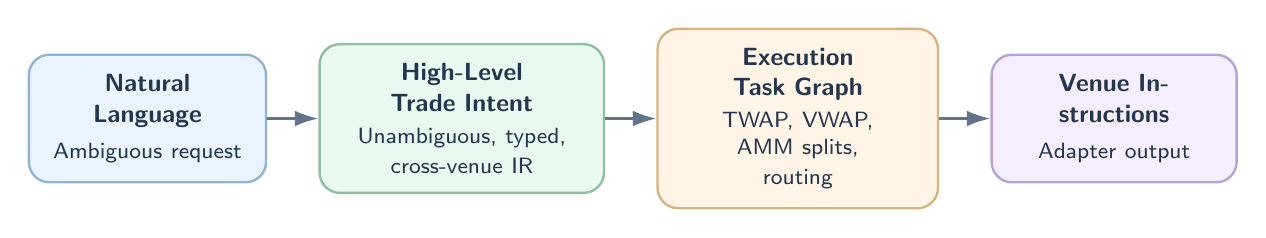
\begin{tikzpicture}[node distance=6.5mm]
  \node[
    stagebox,
    draw=BlueLine,
    fill=BlueFill,
    text width=2.45cm
  ] (nl) {
    \textbf{Natural Language}\\[2pt]
    {\footnotesize Ambiguous request}
  };

  \node[
    stagebox,
    draw=GreenLine,
    fill=GreenFill,
    text width=3.05cm,
    right=of nl
  ] (intent) {
    \textbf{High-Level Trade Intent}\\[2pt]
    {\footnotesize Unambiguous, typed,\\cross-venue IR}
  };

  \node[
    stagebox,
    draw=AmberLine,
    fill=AmberFill,
    text width=3.0cm,
    right=of intent
  ] (tasks) {
    \textbf{Execution Task Graph}\\[2pt]
    {\footnotesize TWAP, VWAP, AMM splits,\\routing}
  };

  \node[
    stagebox,
    draw=PurpleLine,
    fill=PurpleFill,
    text width=2.55cm,
    right=of tasks
  ] (venue) {
    \textbf{Venue Instructions}\\[2pt]
    {\footnotesize Adapter output}
  };

  \draw[flow] (nl.east) -- (intent.west);
  \draw[flow] (intent.east) -- (tasks.west);
  \draw[flow] (tasks.east) -- (venue.west);
\end{tikzpicture}
\end{document}
